% Options for packages loaded elsewhere
\PassOptionsToPackage{unicode}{hyperref}
\PassOptionsToPackage{hyphens}{url}
%
\documentclass[
  english,
  man]{apa6}
\title{Modeling Indoor/Outdoor Images Using Sentence Embeddings}
\author{Anisha Babu\textsuperscript{1}}
\date{}

\usepackage{amsmath,amssymb}
\usepackage{lmodern}
\usepackage{iftex}
\ifPDFTeX
  \usepackage[T1]{fontenc}
  \usepackage[utf8]{inputenc}
  \usepackage{textcomp} % provide euro and other symbols
\else % if luatex or xetex
  \usepackage{unicode-math}
  \defaultfontfeatures{Scale=MatchLowercase}
  \defaultfontfeatures[\rmfamily]{Ligatures=TeX,Scale=1}
\fi
% Use upquote if available, for straight quotes in verbatim environments
\IfFileExists{upquote.sty}{\usepackage{upquote}}{}
\IfFileExists{microtype.sty}{% use microtype if available
  \usepackage[]{microtype}
  \UseMicrotypeSet[protrusion]{basicmath} % disable protrusion for tt fonts
}{}
\makeatletter
\@ifundefined{KOMAClassName}{% if non-KOMA class
  \IfFileExists{parskip.sty}{%
    \usepackage{parskip}
  }{% else
    \setlength{\parindent}{0pt}
    \setlength{\parskip}{6pt plus 2pt minus 1pt}}
}{% if KOMA class
  \KOMAoptions{parskip=half}}
\makeatother
\usepackage{xcolor}
\IfFileExists{xurl.sty}{\usepackage{xurl}}{} % add URL line breaks if available
\IfFileExists{bookmark.sty}{\usepackage{bookmark}}{\usepackage{hyperref}}
\hypersetup{
  pdftitle={Modeling Indoor/Outdoor Images Using Sentence Embeddings},
  pdfauthor={Anisha Babu1},
  pdflang={en-EN},
  pdfkeywords={Natural Language Processing, Scene Images, Modeling},
  hidelinks,
  pdfcreator={LaTeX via pandoc}}
\urlstyle{same} % disable monospaced font for URLs
\usepackage{graphicx}
\makeatletter
\def\maxwidth{\ifdim\Gin@nat@width>\linewidth\linewidth\else\Gin@nat@width\fi}
\def\maxheight{\ifdim\Gin@nat@height>\textheight\textheight\else\Gin@nat@height\fi}
\makeatother
% Scale images if necessary, so that they will not overflow the page
% margins by default, and it is still possible to overwrite the defaults
% using explicit options in \includegraphics[width, height, ...]{}
\setkeys{Gin}{width=\maxwidth,height=\maxheight,keepaspectratio}
% Set default figure placement to htbp
\makeatletter
\def\fps@figure{htbp}
\makeatother
\setlength{\emergencystretch}{3em} % prevent overfull lines
\providecommand{\tightlist}{%
  \setlength{\itemsep}{0pt}\setlength{\parskip}{0pt}}
\setcounter{secnumdepth}{-\maxdimen} % remove section numbering
% Make \paragraph and \subparagraph free-standing
\ifx\paragraph\undefined\else
  \let\oldparagraph\paragraph
  \renewcommand{\paragraph}[1]{\oldparagraph{#1}\mbox{}}
\fi
\ifx\subparagraph\undefined\else
  \let\oldsubparagraph\subparagraph
  \renewcommand{\subparagraph}[1]{\oldsubparagraph{#1}\mbox{}}
\fi
\newlength{\cslhangindent}
\setlength{\cslhangindent}{1.5em}
\newlength{\csllabelwidth}
\setlength{\csllabelwidth}{3em}
\newlength{\cslentryspacingunit} % times entry-spacing
\setlength{\cslentryspacingunit}{\parskip}
\newenvironment{CSLReferences}[2] % #1 hanging-ident, #2 entry spacing
 {% don't indent paragraphs
  \setlength{\parindent}{0pt}
  % turn on hanging indent if param 1 is 1
  \ifodd #1
  \let\oldpar\par
  \def\par{\hangindent=\cslhangindent\oldpar}
  \fi
  % set entry spacing
  \setlength{\parskip}{#2\cslentryspacingunit}
 }%
 {}
\usepackage{calc}
\newcommand{\CSLBlock}[1]{#1\hfill\break}
\newcommand{\CSLLeftMargin}[1]{\parbox[t]{\csllabelwidth}{#1}}
\newcommand{\CSLRightInline}[1]{\parbox[t]{\linewidth - \csllabelwidth}{#1}\break}
\newcommand{\CSLIndent}[1]{\hspace{\cslhangindent}#1}
% Manuscript styling
\usepackage{upgreek}
\captionsetup{font=singlespacing,justification=justified}

% Table formatting
\usepackage{longtable}
\usepackage{lscape}
% \usepackage[counterclockwise]{rotating}   % Landscape page setup for large tables
\usepackage{multirow}		% Table styling
\usepackage{tabularx}		% Control Column width
\usepackage[flushleft]{threeparttable}	% Allows for three part tables with a specified notes section
\usepackage{threeparttablex}            % Lets threeparttable work with longtable

% Create new environments so endfloat can handle them
% \newenvironment{ltable}
%   {\begin{landscape}\centering\begin{threeparttable}}
%   {\end{threeparttable}\end{landscape}}
\newenvironment{lltable}{\begin{landscape}\centering\begin{ThreePartTable}}{\end{ThreePartTable}\end{landscape}}

% Enables adjusting longtable caption width to table width
% Solution found at http://golatex.de/longtable-mit-caption-so-breit-wie-die-tabelle-t15767.html
\makeatletter
\newcommand\LastLTentrywidth{1em}
\newlength\longtablewidth
\setlength{\longtablewidth}{1in}
\newcommand{\getlongtablewidth}{\begingroup \ifcsname LT@\roman{LT@tables}\endcsname \global\longtablewidth=0pt \renewcommand{\LT@entry}[2]{\global\advance\longtablewidth by ##2\relax\gdef\LastLTentrywidth{##2}}\@nameuse{LT@\roman{LT@tables}} \fi \endgroup}

% \setlength{\parindent}{0.5in}
% \setlength{\parskip}{0pt plus 0pt minus 0pt}

% \usepackage{etoolbox}
\makeatletter
\patchcmd{\HyOrg@maketitle}
  {\section{\normalfont\normalsize\abstractname}}
  {\section*{\normalfont\normalsize\abstractname}}
  {}{\typeout{Failed to patch abstract.}}
\patchcmd{\HyOrg@maketitle}
  {\section{\protect\normalfont{\@title}}}
  {\section*{\protect\normalfont{\@title}}}
  {}{\typeout{Failed to patch title.}}
\makeatother
\shorttitle{Modeling Scene Images}
\keywords{Natural Language Processing, Scene Images, Modeling}
\DeclareDelayedFloatFlavor{ThreePartTable}{table}
\DeclareDelayedFloatFlavor{lltable}{table}
\DeclareDelayedFloatFlavor*{longtable}{table}
\makeatletter
\renewcommand{\efloat@iwrite}[1]{\immediate\expandafter\protected@write\csname efloat@post#1\endcsname{}}
\makeatother
\usepackage{csquotes}
\ifXeTeX
  % Load polyglossia as late as possible: uses bidi with RTL langages (e.g. Hebrew, Arabic)
  \usepackage{polyglossia}
  \setmainlanguage[]{english}
\else
  \usepackage[main=english]{babel}
% get rid of language-specific shorthands (see #6817):
\let\LanguageShortHands\languageshorthands
\def\languageshorthands#1{}
\fi
\ifLuaTeX
  \usepackage{selnolig}  % disable illegal ligatures
\fi


\affiliation{\vspace{0.5cm}\textsuperscript{1} University of Oregon}

\begin{document}
\maketitle

\hypertarget{reproducibility}{%
\section{Reproducibility:}\label{reproducibility}}

Link to the GitHub repo: \url{https://github.com/anishababu62442/EDLD654-Final}

\hypertarget{research-problem}{%
\section{Research problem:}\label{research-problem}}

As we navigate the world, we continuously form memories of similar events. However, similarity between memories can lead to interference (Mensink and Raaijmakers (1988); O'Reilly and McClelland (1994)). For example, remembering a password for one account is often complicated by interference from memories of other passwords. Although there have been many studies on memory interference, they have primarily focused on the fact that similarity reduces the probability of successfully remembering an event. Meanwhile, an under-explored question is whether similarity changes memories. On the one hand, similarity may lead to integration of similar memories, such that two memories blend together. On the other hand, similarity may lead to repulsion, wherein information that differentiates similar events becomes prioritized in memory (Hulbert and Norman (2015)) or even exaggerated (Chanales, Tremblay-McGaw, Drascher, and Kuhl (2021)). For example, let's say you visited the same restaurant on two different days: a sunny day in August and a breezy day in September. If memory integration occurs, you may blend details of the events (a sunny day in September). If memory repulsion occurs, your memories may prioritize details that differed across the two events (the weather) or even exaggerate differences (a particularly windy day in September). This example illustrates that similarity between events may shape how they are remembered. Critically, these changes, or distortions, in memory content are potentially systematic and, therefore, predictable.

Ultimately, I will test for similarity-induced changes in memory content using innovative behavioral methods. Specifically, I will use Natural Language Processing (NLP) techniques to determine whether and how similarity induces changes in memory content. My overarching hypothesis is that similarity between memories will lead to predictable distortions in memory content.

In this paper, I will assess preliminary data that will determine the feasibility of using NLP in a full-scale study. NLP is a powerful tool for transforming natural language into numerical vectors that represent semantic information across hundreds of dimensions. Translating memories into these numerical feature spaces will allow me to mathematically express content similarity between individual memories. However, in order to measure how similar memories change, I must first establish a baseline to which written memory can be compared.

The stimuli that were used in this preliminary experiment will be used in subsequent memory experiments as well. They consist of a set of naturalistic scene images, with 15 exemplars from 30 categories (e.g., 15 beaches, 15 airports, 15 libraries, etc.). Critically, 15 categories were indoor scenes, and 15 categories were outdoor scenes. In this experiment, participants viewed one image from each category, and wrote a description underneath in at least 15 words. This experiment did not involve a memory task and participants were not exposed to any similar images (i.e., no images from the same category). The purpose of this experiment is to generate baseline vectors using NLP that represent the content of each scene image. Subsequent experiments will compare remembered content to these baseline vectors. See below some sample responses:

\begin{tabular}{l|>{\raggedright\arraybackslash}p{25em}}
\hline
Image & Description\\
\hline
Ice-skating rink & Ice rink filled with families, children and adults. Two men, and two children hold hands in a row of four. It is a least chilly with many wearing hats, and warm coats.\\
\hline
Library & a library, which is similar to that of trinity college belfast, rows of brown bookshelves filled with old leather bound books. at the end of the corridor a large partly stained glass window. The ceiling is highly decora\\
\hline
Indoor pool & An almost empty, modernist indoor pooL with sliding glass windows around the entire building and multiple skylights. Four beach chairs at the end of the pool, to the right a gie\\
\hline
Train station & Train pulls into a staion, the time is just after 6.10pm, a woman in a mask looks at the train. The station is filled with one other person, sat on a bench. It appears to be a fairly old station metal\\
\hline
Arcade & Arcade, lit only by the various machines, these are mostly ball games for prizes instead of the usual video games often depicted. It has a styrofoam ceiling. The lights are purple, blue, and green in neon.\\
\hline
\end{tabular}

At the end of the experiment, I had a set of five descriptions for each of the 450 images (30 categories x 15 exemplars). Each of these descriptions was transformed into numerical vectors using the NLP algorithm MPNet (Song, Tan, Qin, Lu, and Liu (2020)). In this paper, I will assess the specificity of these vectors using machine learning techniques. Specifically, I seek to classify descriptions as corresponding to either an indoor or outdoor image. This analysis will reveal the ability to extrapolate semantic information from MPNet output. Rather than classifying descriptions into specific categories (which are often explicitly written in descriptions), classifying indoor/outdoor images will allow for an interesting assessment of NLP techniques more generally. If successful, this would indicate NLP is a feasible method for quantifying written memory in future experiments. It would be especially interesting to see if a model trained on this baseline data is successful in classifying data from a memory experiment.

\hypertarget{description-of-the-data}{%
\section{Description of the data:}\label{description-of-the-data}}

As described before, there were a total of 30 scene image categories, each with 15 images. Critically, half of these categories were outdoor scenes, and half of these categories were indoor scenes.

Using separate Python code, written descriptions were transformed into 768-dimension numerical vectors using MPNet. Each description also includes a marker for whether the description corresponds to either an indoor or outdoor image. See first seven columns of sample data:

\begin{tabular}{l|r|r|r|r|r|r}
\hline
Location & V1 & V2 & V3 & V4 & V5 & V6\\
\hline
Indoor & -0.0630010 & -0.0864007 & 0.0056232 & 0.2349402 & 0.0210362 & 0.0293891\\
\hline
Indoor & 0.0555179 & 0.0459704 & 0.0075291 & 0.0934091 & -0.2211835 & 0.1114800\\
\hline
Indoor & -0.1413176 & -0.2072940 & 0.1051668 & -0.0065399 & -0.0954954 & -0.0198655\\
\hline
Outdoor & -0.1735294 & 0.0211764 & 0.0929864 & 0.1799997 & 0.0699336 & -0.0089860\\
\hline
Indoor & 0.0804916 & -0.0159084 & 0.0089862 & 0.2014005 & -0.1113927 & 0.0549167\\
\hline
\end{tabular}

See below for count of indoor/outdoor images:

\begin{tabular}{l|r}
\hline
Var1 & Freq\\
\hline
Indoor & 1125\\
\hline
Outdoor & 1125\\
\hline
\end{tabular}

\hypertarget{description-of-the-models}{%
\section{Description of the models:}\label{description-of-the-models}}

The first modeling approach I used is logistic regression. I chose this model rather than linear regression because I have a binary outcome (indoor/outdoor), and the model assumptions require a binary outcome. We can also assume the 768 variables outputted from MPNet are independent of one another. To select a model version, I assessed a model without penalty, a model with ridge penalty, and a model with lasso penalty. The cutoff for predictions is: probability \textgreater{} 0.5. For the ridge penalty and lasso penalty versions, multiple lambda values were assessed to find the best fit. The best performing model will be chosen based on measures of: area under the curve, accuracy, and precision.

The second modeling approach I used is a decision tree. NLP output includes hundreds of dimensions representing semantic information. However, it is unlikely that all dimensions are relevant in determining if an image was indoor or outdoor. As such, a decision tree is useful in that it selects the most important variable dimensions, and classifies samples based on values along those important dimensions. The cutoff probability for predictions is: probability \textgreater{} 0.5. To find the best complexity parameter, multiple values were assessed. The model will be assessed based on measures of: area under the curve, accuracy, and precision.

The third modeling approach I used is a bagged tree model. This model randomly selects from the 2250 samples and makes aggregate predictions for multiple different trees. The cutoff probability for predictions is: probability \textgreater{} 0.5. To select the best number of trees, I assessed different numbers from 1-200. The model will be assessed based on measures of: area under the curve, accuracy, and precision.

\hypertarget{model-fit}{%
\section{Model fit:}\label{model-fit}}

For the logistic regression model, I tried three different versions: without penalty, with ridge penalty, and with lasso penalty. For ridge penalty, I tested multiple lambda values as seen in the figure below.

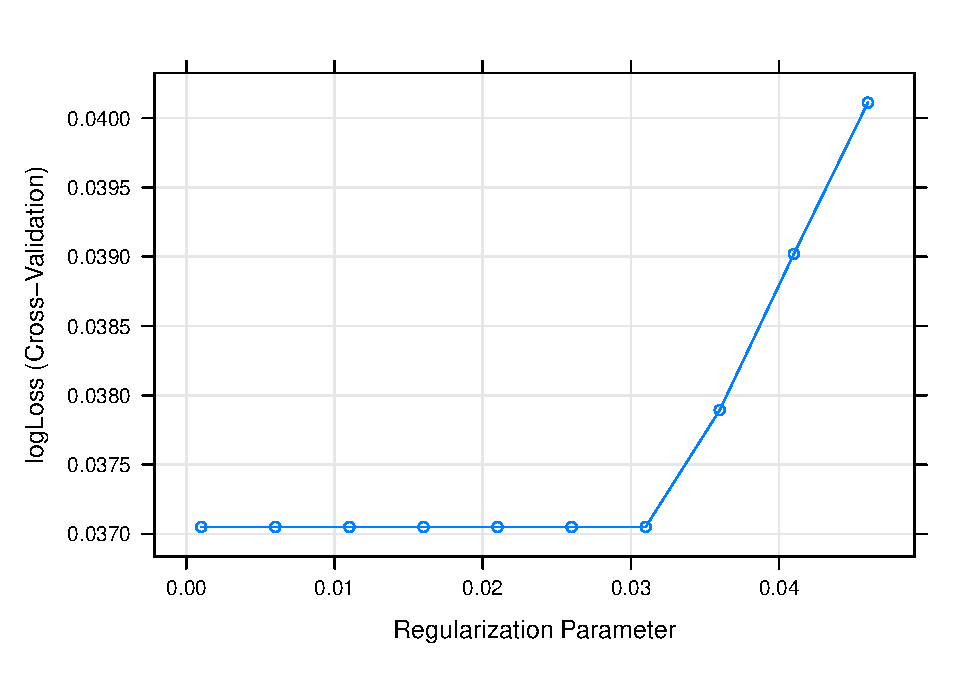
\includegraphics{Babu_Final_files/figure-latex/ridge log-1.pdf}

For lasso penalty, I tested multiple lambda values as seen in the figure below.

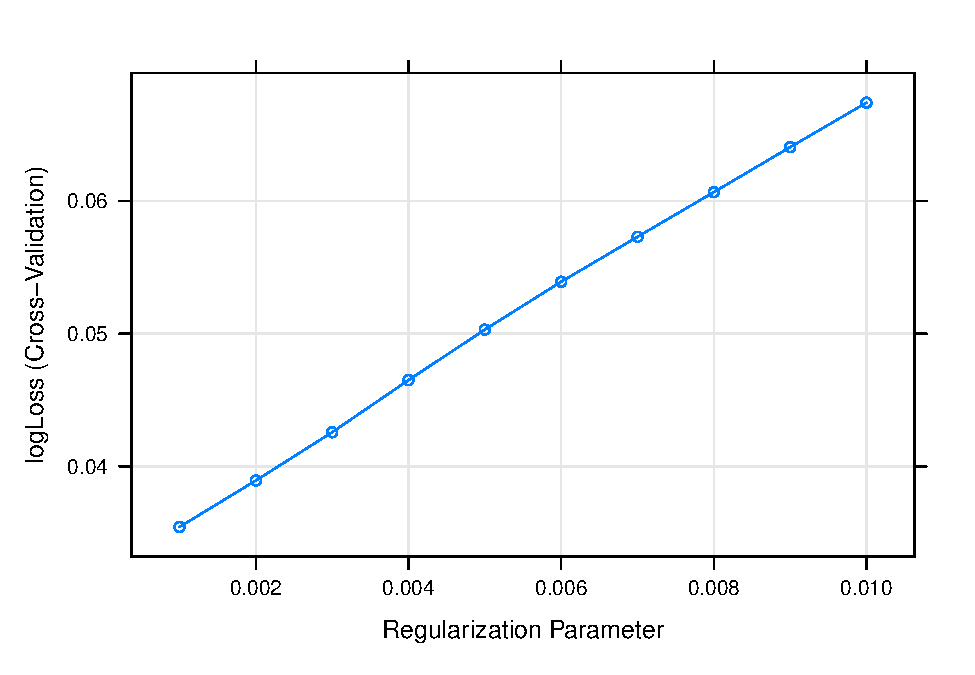
\includegraphics{Babu_Final_files/figure-latex/lasso log-1.pdf}

I assessed performance for each version by calculating area under the curve, accuracy, and precision (summarized in table below). Based on these results, I would choose logistic regression with ridge penalty, as it had the highest accuracy and precision, and close to the highest area under the curve. Strikingly, all models have very high performance overall.

\begin{tabular}{l|r|r|r|r|r|r}
\hline
  & LL & AUC & ACC & TPR & TNR & PRE\\
\hline
Log Reg & 0.1740108 & 0.9994863 & 0.9911111 & 0.9954955 & 0.9868421 & 0.9866071\\
\hline
Log Reg with Ridge & 0.0370500 & 0.9994666 & 0.9955556 & 1.0000000 & 0.9912281 & 0.9910714\\
\hline
Log Reg with Lasso & 0.0354410 & 0.9994468 & 0.9911111 & 0.9954955 & 0.9868421 & 0.9866071\\
\hline
\end{tabular}

For the decision tree model, I tested multiple complexity parameter values as seen in the figure below.

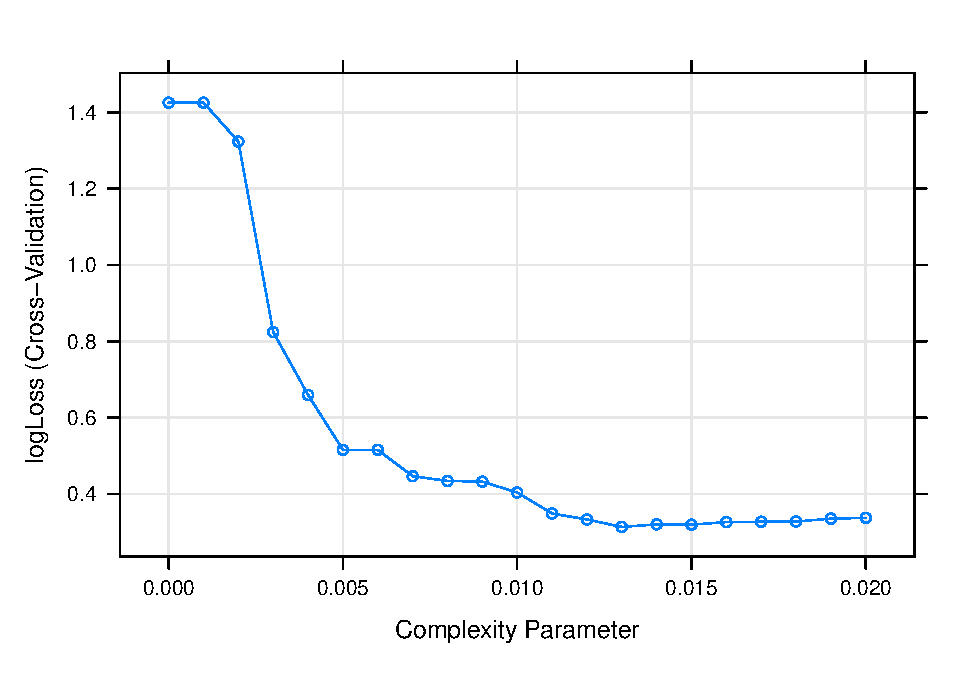
\includegraphics{Babu_Final_files/figure-latex/descision model-1.pdf}

See figure below for diagram of decision tree. I also assessed performance for the decision tree model by calculating area under the curve, accuracy, and precision (summarized in table at the end).

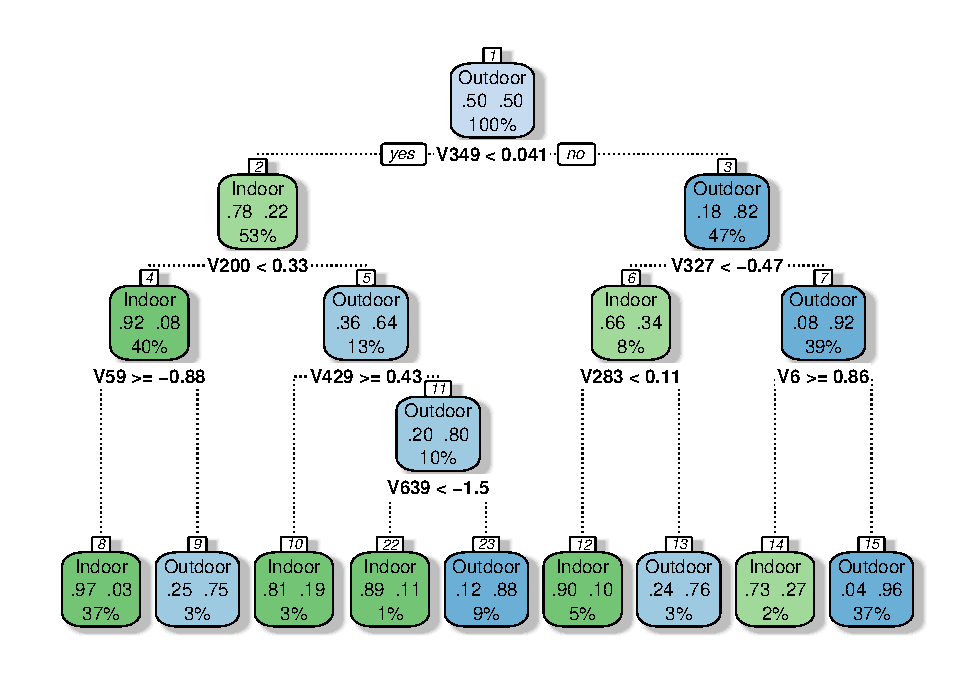
\includegraphics{Babu_Final_files/figure-latex/show tree-1.pdf}

For the bagged tree model, I tested multiple number of tree values (1-200). Due to high computational time, the figure below shows only a few sample values. I also assessed performance for the bagged tree model by calculating area under the curve, accuracy, and precision (summarized in table at the end).

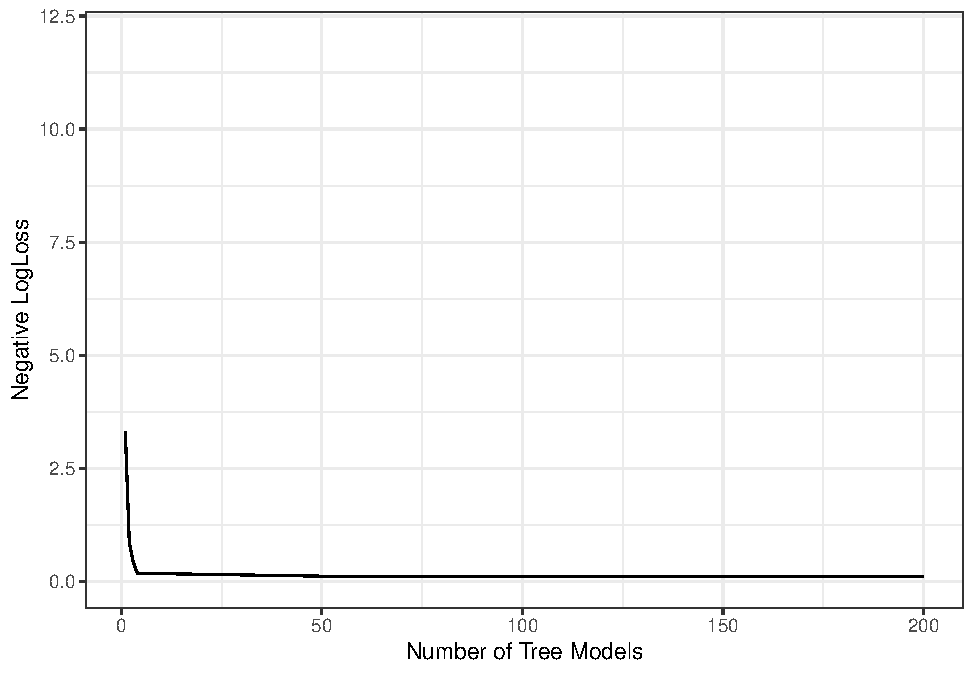
\includegraphics{Babu_Final_files/figure-latex/best bagged-1.pdf}

The table below shows results for all three models considered based on measures of area under the curve, accuracy, and precision. From these measures, logistic regression with ridge regression performs the best, followed by the bagged tree model, then the decision tree model.

\begin{tabular}{l|r|r|r|r|r|r}
\hline
  & LL & AUC & ACC & TPR & TNR & PRE\\
\hline
Log Reg with Ridge & 0.0370500 & 0.9994666 & 0.9955556 & 1.0000000 & 0.9912281 & 0.9910714\\
\hline
Decision Tree & 0.3135789 & 0.9416390 & 0.9000000 & 0.9144144 & 0.8859649 & 0.8864629\\
\hline
Bagged Tree & 0.1141214 & 0.9984491 & 0.9844444 & 0.9954955 & 0.9736842 & 0.9735683\\
\hline
\end{tabular}

\hypertarget{discussionconclusion}{%
\section{Discussion/Conclusion:}\label{discussionconclusion}}

It was interesting to find that, despite using more complex models like decision trees and bagged trees, logistic regression still had the best performance. Since the variables used were NLP output, we do not actually know what information specific variables represent. As such, the variables used in the decision tree are interesting in that they show which of the 768 NLP output values may represent indoor/outdoor information.
The decision tree performed noticeably poorer compared to the logistic regression and bagged tree models. This may be because decision tree models are better suited to categorical values, and when used here had to be limited whether the variable is greater than or less than some value.
These findings are useful in showing that overall, there was quite high accuracy in decoding whether images were indoor or outdoor. This suggests the written image descriptions are descriptive enough that they may prove useful in a future memory experiment.

\newpage

\hypertarget{references}{%
\section{References}\label{references}}

\begingroup
\setlength{\parindent}{-0.5in}
\setlength{\leftskip}{0.5in}

\hypertarget{refs}{}
\begin{CSLReferences}{1}{0}
\leavevmode\vadjust pre{\hypertarget{ref-chanales2021}{}}%
Chanales, A. J., Tremblay-McGaw, A., Drascher, M., \& Kuhl, B. A. (2021). Adaptive repulsion of long- term memory representations is triggered by event similarity. \emph{Psychological Science}, \emph{32}, 705--720.

\leavevmode\vadjust pre{\hypertarget{ref-hulbert2015}{}}%
Hulbert, J. C., \& Norman, K. A. (2015). Neural differentiation tracks improved recall of competing memories following interleaved study and retrieval practice. \emph{Cerebral Cortex}, \emph{25}(10), 3994--4008.

\leavevmode\vadjust pre{\hypertarget{ref-mensink1988}{}}%
Mensink, G. M., \& Raaijmakers, J. G. (1988). The production of social capital in US counties. \emph{Psychological Review}, \emph{95}, 434--455.

\leavevmode\vadjust pre{\hypertarget{ref-oreilly1994}{}}%
O'Reilly, R. C., \& McClelland, J. L. (1994). Hippocampal conjunctive encoding, storage, and recall: Avoiding a trade-off. \emph{Hippocampus}, \emph{4}(6), 661--682.

\leavevmode\vadjust pre{\hypertarget{ref-song2020}{}}%
Song, K., Tan, X., Qin, T., Lu, J., \& Liu, T. (2020). MPNet: Masked and permuted pre-training for language understanding. \emph{ArXiv}.

\end{CSLReferences}

\endgroup


\end{document}
